\chapter{Privacy-Preserving Anomaly Detection: Implementation and Results}
\chaptermark{Implementation and Results}
\HRule\\[2cm]
\label{Chapter5}
\lhead{\emph{\textbf{Chapter 5:} Implementation and Results}}

\begin{spacing}{1.6}

% ─────────────────────────────────────────────────────────────
\section{HE-SAD: Homomorphic Statistical Anomaly Detection}
% ─────────────────────────────────────────────────────────────

\subsection{Algorithm Design Under CKKS Constraints}

The SAD anomaly score (Equation~\ref{eq:sad}) decomposes into four operations
that must be executed under CKKS encryption for each test ciphertext:

\begin{enumerate}
  \item \textbf{Centering:} Subtract the plaintext mean vector from the
  encrypted test row. Since $\boldsymbol{\mu}$ is a plaintext vector (computed
  from the multi-round protocol result and known to the server), this is a
  \texttt{sub\_plain} operation.
  \begin{equation}
    \mathrm{ct}_{xc} \leftarrow \mathrm{ct}_i - \mathrm{pt}_\mu
    \quad \text{(0 levels consumed)}
  \end{equation}

  \item \textbf{Squaring:} Square the centred ciphertext element-wise to
  compute $(x_j - \mu_j)^2$ for all $j$ simultaneously.
  \begin{equation}
    \mathrm{ct}_{sq} \leftarrow \mathrm{ct}_{xc}^2
    \xrightarrow{\text{relinearize}} \xrightarrow{\text{rescale}}
    \quad \text{(1 level consumed)}
  \end{equation}
  After squaring, the ciphertext scale doubles to $2^{80}$. Relinearization
  reduces the degree-2 result back to degree-1 format. Rescaling divides by
  the last prime in the modulus chain, returning to scale $2^{40}$ and
  consuming one level.

  \item \textbf{Variance normalisation:} Multiply element-wise by the
  plaintext vector of inverse variances $1/\sigma_j^2$.
  \begin{equation}
    \mathrm{ct}_{sc} \leftarrow \mathrm{ct}_{sq} \cdot
    \mathrm{pt}_{1/\sigma^2}
    \xrightarrow{\text{rescale}}
    \quad \text{(1 level consumed)}
  \end{equation}
  The plaintext $\mathrm{pt}_{1/\sigma^2}$ must be encoded at the
  ciphertext's current scale to avoid scale mismatch errors.

  \item \textbf{Slot summation:} Sum all $d$ slot values to obtain the
  scalar anomaly score in slot~0.
  \begin{equation}
    \mathrm{ct}_{score} \leftarrow
    \sum_{k=0}^{\lceil\log_2 d\rceil - 1}
    \mathrm{Rot}(\mathrm{ct}_{sc}, 2^k) + \mathrm{ct}_{sc}
    \quad \text{(0 levels, 6 rotations)}
  \end{equation}
  The binary rotation tree sums $d$ slot values using
  $\lceil\log_2 d\rceil$ rotate-and-add steps.
  Zero-padded slots contribute nothing to the sum.
\end{enumerate}

Table~\ref{tab:sad_depth} summarises the HE depth consumed per test row.

\end{spacing}

\begin{table}[!ht]
\centering
\caption{HE-SAD Per-Row Computation Depth Budget (5 levels available)}
\label{tab:sad_depth}
\begin{tabular}{p{4cm}p{5cm}cc}
\toprule
\textbf{Operation} & \textbf{SEAL Method} & \textbf{Levels} & \textbf{Rotations} \\
\midrule
$\mathbf{x}_i - \boldsymbol{\mu}$ &
  \texttt{sub\_plain(ct\_i, pt\_mu)} & 0 & 0 \\
$(x_j - \mu_j)^2$ &
  \texttt{square}, \texttt{relinearize}, \texttt{rescale} & 1 & 0 \\
$\times\,1/\sigma_j^2$ &
  \texttt{multiply\_plain}, \texttt{rescale} & 1 & 0 \\
$\sum_{j=1}^{d}$ &
  \texttt{rotate\_and\_add} $\times\,\lceil\log_2 d\rceil$ & 0 & 6 \\
\midrule
\textbf{Total per row} & & \textbf{2 of 5} & \textbf{6} \\
\bottomrule
\end{tabular}
\end{table}

\begin{spacing}{1.6}

\subsection{The Nine-Round HE-SAD Protocol}

The complete protocol is shown in Table~\ref{tab:sad_proto}, and the full
client--server state-transition diagram is presented in
Figure~\ref{fig:sad_protocol}.

\end{spacing}

\begin{table}[!ht]
\centering
\caption{Complete HE-SAD Protocol}
\label{tab:sad_proto}
\begin{tabular}{p{0.6cm}p{2.8cm}p{7.2cm}p{2.5cm}}
\toprule
\textbf{Rnd} & \textbf{Operation} & \textbf{Details} & \textbf{Direction} \\
\midrule
1 & Upload training data &
  Column-major ciphertexts ($\approx$51\,MB); one per feature with all
  $N$ training row values in SIMD slots &
  Client $\to$ Server \\[4pt]
2 & Compute column sums &
  Server applies binary rotation tree (13 rotations per feature);
  returns $\mathrm{ct}_N$ encoding $N$ in all slots &
  Server $\to$ Client \\[4pt]
3 & Invert $N$ &
  Client decrypts $\mathrm{ct}_N$, computes exact $1/N$ in plaintext,
  re-encrypts as $\mathrm{ct}_{1/N}$ &
  Client $\to$ Server \\[4pt]
4 & Compute $\mu$ and $\sigma^2$ &
  Server computes $\mathrm{ct}_{\mu_j} = \mathrm{ct}_{\mathrm{sum},j}
  \cdot \mathrm{ct}_{1/N}$; derives $\mathrm{ct}_{\sigma^2_j}$ from
  training ciphertexts; sends packed $\mathrm{ct}_{\sigma^2}$ to client &
  Server $\to$ Client \\[4pt]
5 & Invert $\sigma^2$ &
  Client decrypts all $d$ variance values; computes exact
  $1/\sigma_j^2$; re-encrypts as packed $\mathrm{ct}_{1/\sigma^2}$ &
  Client $\to$ Server \\[4pt]
6 & Upload test data &
  Row-major ciphertexts uploaded in batches of 100 per HTTP POST
  ($\approx$100\,MB per batch) &
  Client $\to$ Server \\[4pt]
7 & Compute SAD scores &
  Server scores all test ciphertexts asynchronously in a background
  thread; 2 HE levels consumed per row &
  Server (async) \\[4pt]
8 & Fetch scores &
  Client polls \texttt{/api/scores/status} every 5\,s; fetches
  encrypted scores in batches of 100 &
  Server $\to$ Client \\[4pt]
9 & Decrypt and classify &
  Client decrypts all score ciphertexts using $\mathbf{sk}$; applies
  threshold $\tau = \bar{s}_\mathrm{train} + 3\sigma_{s,\mathrm{train}}$;
  computes AUC, F1, Precision, Recall &
  Client (local) \\
\bottomrule
\end{tabular}
\end{table}

\begin{figure}[!ht]
\centering
\includegraphics[width=\textwidth]{Images/he_sad_protocol.png}
\caption{HE-SAD nine-round protocol: full client--server state-transition
diagram showing internal state flow within each party and cross-network
message exchanges. The server holds only ciphertexts and public keys;
the secret key $\mathbf{sk}$ never leaves the client.}
\label{fig:sad_protocol}
\end{figure}

\begin{spacing}{1.6}

\subsection{Threshold Computation}

The detection threshold $\tau$ is computed from the normal training data
using the same HE-SAD scoring function:
\begin{equation}
  \tau = \bar{s}_\mathrm{train} + 3\,\sigma_{s,\mathrm{train}}
\end{equation}
Training rows are encrypted and scored through the live HE-SAD computation,
ensuring the threshold is calibrated to the actual HE score distribution
(which may differ slightly from plaintext SAD scores due to bounded CKKS
approximation noise $\approx 10^{-9}$) rather than to plaintext scores.

% ─────────────────────────────────────────────────────────────
\section{HE-PCA: Homomorphic Principal Component Analysis}
% ─────────────────────────────────────────────────────────────

\subsection{Algorithm Design Under CKKS Constraints}

The PCA reconstruction error (Equation~\ref{eq:pca}) requires five
operations per encrypted test row:

\begin{enumerate}
  \item \textbf{Centering:}
  \begin{equation}
    \mathrm{ct}_{xc} \leftarrow \mathrm{ct}_i - \mathrm{pt}_\mu
    \quad\text{(0 levels)}
  \end{equation}

  \item \textbf{Projection onto each component $k$:}
  \begin{equation}
    p_k = \langle \mathrm{ct}_{xc},\,\mathbf{v}_k \rangle
        = \mathrm{slot\_sum}\!\left(
            \mathrm{ct}_{xc} \cdot \mathrm{pt}_{\mathbf{v}_k}
          \right)
    \quad\text{(1 level)}
  \end{equation}

  \item \textbf{Reconstruction of component $k$:}
  \begin{equation}
    \mathrm{ct}_{r_k} = p_k \cdot \mathrm{pt}_{\mathbf{v}_k}
    \quad\text{(1 level)}
  \end{equation}
  The scalar $p_k$ (in slot~0 after the slot sum) is broadcast to all
  slots via a \texttt{multiply\_plain} with $\mathbf{v}_k$.

  \item \textbf{Residual:}
  \begin{equation}
    \mathrm{ct}_{res} = \mathrm{ct}_{xc}
      - \sum_{k=1}^{k^*} \mathrm{ct}_{r_k}
    \quad\text{(0 levels)}
  \end{equation}

  \item \textbf{Squared residual norm:}
  \begin{equation}
    \mathrm{ct}_{score} =
      \mathrm{slot\_sum}\!\left(\mathrm{ct}_{res}^2\right)
    \quad\text{(1 level + 6 rotations)}
  \end{equation}
\end{enumerate}

Table~\ref{tab:pca_depth} summarises the HE depth consumed per test row.

\end{spacing}

\begin{table}[!ht]
\centering
\caption{HE-PCA Per-Row Computation Depth Budget (5 levels available)}
\label{tab:pca_depth}
\begin{tabular}{p{4cm}p{5cm}cc}
\toprule
\textbf{Operation} & \textbf{SEAL Method} & \textbf{Levels} & \textbf{Rotations} \\
\midrule
$\mathbf{x}_i - \boldsymbol{\mu}$ &
  \texttt{sub\_plain} & 0 & 0 \\
$\langle\mathrm{ct}_{xc},\mathbf{v}_k\rangle$ &
  \texttt{multiply\_plain} + \texttt{rescale} + \texttt{slot\_sum} & 1 & 6 \\
$p_k \cdot \mathbf{v}_k$ &
  \texttt{multiply\_plain} + \texttt{rescale} & 1 & 0 \\
Residual &
  \texttt{sub} $\times\,k^*$ & 0 & 0 \\
$\|\mathrm{ct}_{res}\|^2$ &
  \texttt{square} + \texttt{rescale} + \texttt{slot\_sum} & 1 & 6 \\
\midrule
\textbf{Total per row} & & \textbf{3 of 5} & \textbf{12} \\
\bottomrule
\end{tabular}
\end{table}

\begin{spacing}{1.6}

\subsection{Optimal Component Selection}

The number of principal components $k^*$ is selected automatically using
the 90\% explained variance threshold:
\begin{equation}
  k^* = \min\!\left\{k :\;
    \frac{\sum_{i=1}^{k}\lambda_i}{\sum_{i=1}^{d}\lambda_i}
    \geq 0.90\right\}
\end{equation}
The server fits a full PCA on the plaintext training CSV (a public model
parameter, not individual data) and selects $k^*$ automatically.
Only the integer $k^*$ and the achieved variance ratio are reported to the
client; no raw feature values are revealed.

\subsection{The Eight-Round HE-PCA Protocol}

The complete protocol is shown in Table~\ref{tab:pca_proto}, and the full
client--server state-transition diagram is presented in
Figure~\ref{fig:pca_protocol}.

\end{spacing}

\begin{table}[!ht]
\centering
\caption{Complete HE-PCA Protocol}
\label{tab:pca_proto}
\begin{tabular}{p{0.6cm}p{2.8cm}p{7.2cm}p{2.5cm}}
\toprule
\textbf{Rnd} & \textbf{Operation} & \textbf{Details} & \textbf{Direction} \\
\midrule
1 & Upload training data &
  Column-major ciphertexts; one per feature &
  Client $\to$ Server \\[4pt]
2 & Compute column sums &
  Binary rotation tree; returns $\mathrm{ct}_N$ &
  Server $\to$ Client \\[4pt]
3 & Invert $N$ &
  Exact $1/N$ plaintext inversion and re-encryption &
  Client $\to$ Server \\[4pt]
4 & Compute $\mu$ and fit PCA &
  Server computes $\mathrm{ct}_\mu$ using $\mathrm{ct}_{1/N}$;
  fits PCA on plaintext training CSV;
  selects $k^*$ via 90\% variance threshold;
  stores component matrix $\mathbf{V}_{k^*}$ as server state &
  Server (internal) \\[4pt]
5 & Upload test data &
  Row-major ciphertexts in batches of 100 per POST request &
  Client $\to$ Server \\[4pt]
6 & Compute PCA scores &
  Server scores all test ciphertexts asynchronously;
  $2k^*$ multiply\_plain + rescale operations per row;
  3 HE levels consumed &
  Server (async) \\[4pt]
7 & Fetch scores &
  Client polls every 5\,s; fetches score cts in batches of 100 &
  Server $\to$ Client \\[4pt]
8 & Decrypt and classify &
  Client decrypts, applies threshold, computes metrics &
  Client (local) \\
\bottomrule
\end{tabular}
\end{table}

\begin{figure}[!ht]
\centering
\includegraphics[width=\textwidth]{Images/he_pca_protocol.png}
\caption{HE-PCA eight-round protocol: full client--server state-transition
diagram. The component matrix $\mathbf{V}$ is a plaintext model parameter
fitted on the training CSV; no individual data point is revealed to the
server at any step.}
\label{fig:pca_protocol}
\end{figure}

\begin{spacing}{1.6}

% ─────────────────────────────────────────────────────────────
\section{Network Architecture and API Design}
% ─────────────────────────────────────────────────────────────

\subsection{REST API Design}

The detection server exposes 14 REST endpoints via FastAPI, summarised in
Table~\ref{tab:api}.

\end{spacing}

\begin{table}[!ht]
\centering
\caption{FastAPI Server REST Endpoints}
\label{tab:api}
\begin{tabular}{llp{7cm}}
\toprule
\textbf{Method} & \textbf{Endpoint} & \textbf{Purpose} \\
\midrule
POST & \texttt{/api/reset} &
  Initialise \texttt{ServerState}; set SAD or PCA mode \\
POST & \texttt{/api/upload/train} &
  Receive training ciphertexts \\
GET  & \texttt{/api/compute/sum} &
  Compute column sums; return $\mathrm{ct}_N$ \\
POST & \texttt{/api/invert/N} &
  Receive $\mathrm{ct}_{1/N}$ from client \\
GET  & \texttt{/api/compute/mu} &
  Compute $\boldsymbol{\mu}$; fit PCA if PCA mode \\
POST & \texttt{/api/invert/sigma2} &
  Receive $\mathrm{ct}_{1/\sigma^2}$ (SAD only) \\
POST & \texttt{/api/upload/test} &
  Receive test ciphertexts (batch of 100) \\
GET  & \texttt{/api/compute/scores} &
  Trigger async background score computation \\
GET  & \texttt{/api/scores/status} &
  Poll scoring progress \\
GET  & \texttt{/api/scores/batch} &
  Fetch encrypted scores (batch of 100) \\
POST & \texttt{/api/results} &
  Client posts final classification metrics \\
GET  & \texttt{/api/results} &
  Dashboard reads final metrics \\
GET  & \texttt{/api/status} &
  Round number, timing, PCA component count \\
GET  & \texttt{/api/health} &
  Health check \\
\bottomrule
\end{tabular}
\end{table}

\begin{spacing}{1.6}

\subsection{Batched Ciphertext Transfer}

Each SEAL ciphertext with polynomial modulus degree 16384 and coefficient
modulus $[60,40,40,40,40,40,60]$ serialises to approximately 1\,MB on disk.
The test and training ciphertexts therefore total approximately 2.05\,GB.
Attempting to transmit all test ciphertexts in a single HTTP request exceeds
the operating system socket buffer, causing a connection error. The solution
is to transfer ciphertexts in batches of 100 per HTTP request
($\approx$100\,MB each), which the server appends to a unified list.

\subsection{Asynchronous Score Computation}

HE-PCA scoring over many component projections can exceed the 300\,s default
HTTP timeout if run synchronously. The solution launches scoring in a
\texttt{threading.Thread} and returns an immediate acknowledgement. The client
polls \texttt{/api/scores/status} every 5\,s until the response indicates
\texttt{"status": "ready"}, then fetches score ciphertexts in batches of 100.
The scoring timeout is configurable (\texttt{SCORE\_TIMEOUT = 3600}\,s).

\subsection{Live Monitoring Dashboard}

The monitoring dashboard provides real-time observability of the
privacy-preserving detection pipeline. Figure~\ref{fig:dashboard_overview}
shows the control panel and activity log during HE-SAD execution.
Figure~\ref{fig:dashboard_results} shows the results view after protocol
completion.

\textbf{Control panel:} Send Data (with progress bar), Pause/Resume, Stop,
Run SAD, Run PCA, Reset.

\textbf{Monitoring displays:} scrolling timestamped activity log; round
status checklist with per-round latency; latency bar chart; throughput in
rows/second; AUC, F1, Precision, Recall; colour-coded confusion matrix;
score distribution histogram with threshold line; PCA component card
showing $k^*$ and variance explained.

\end{spacing}

\begin{figure}[!ht]
\centering
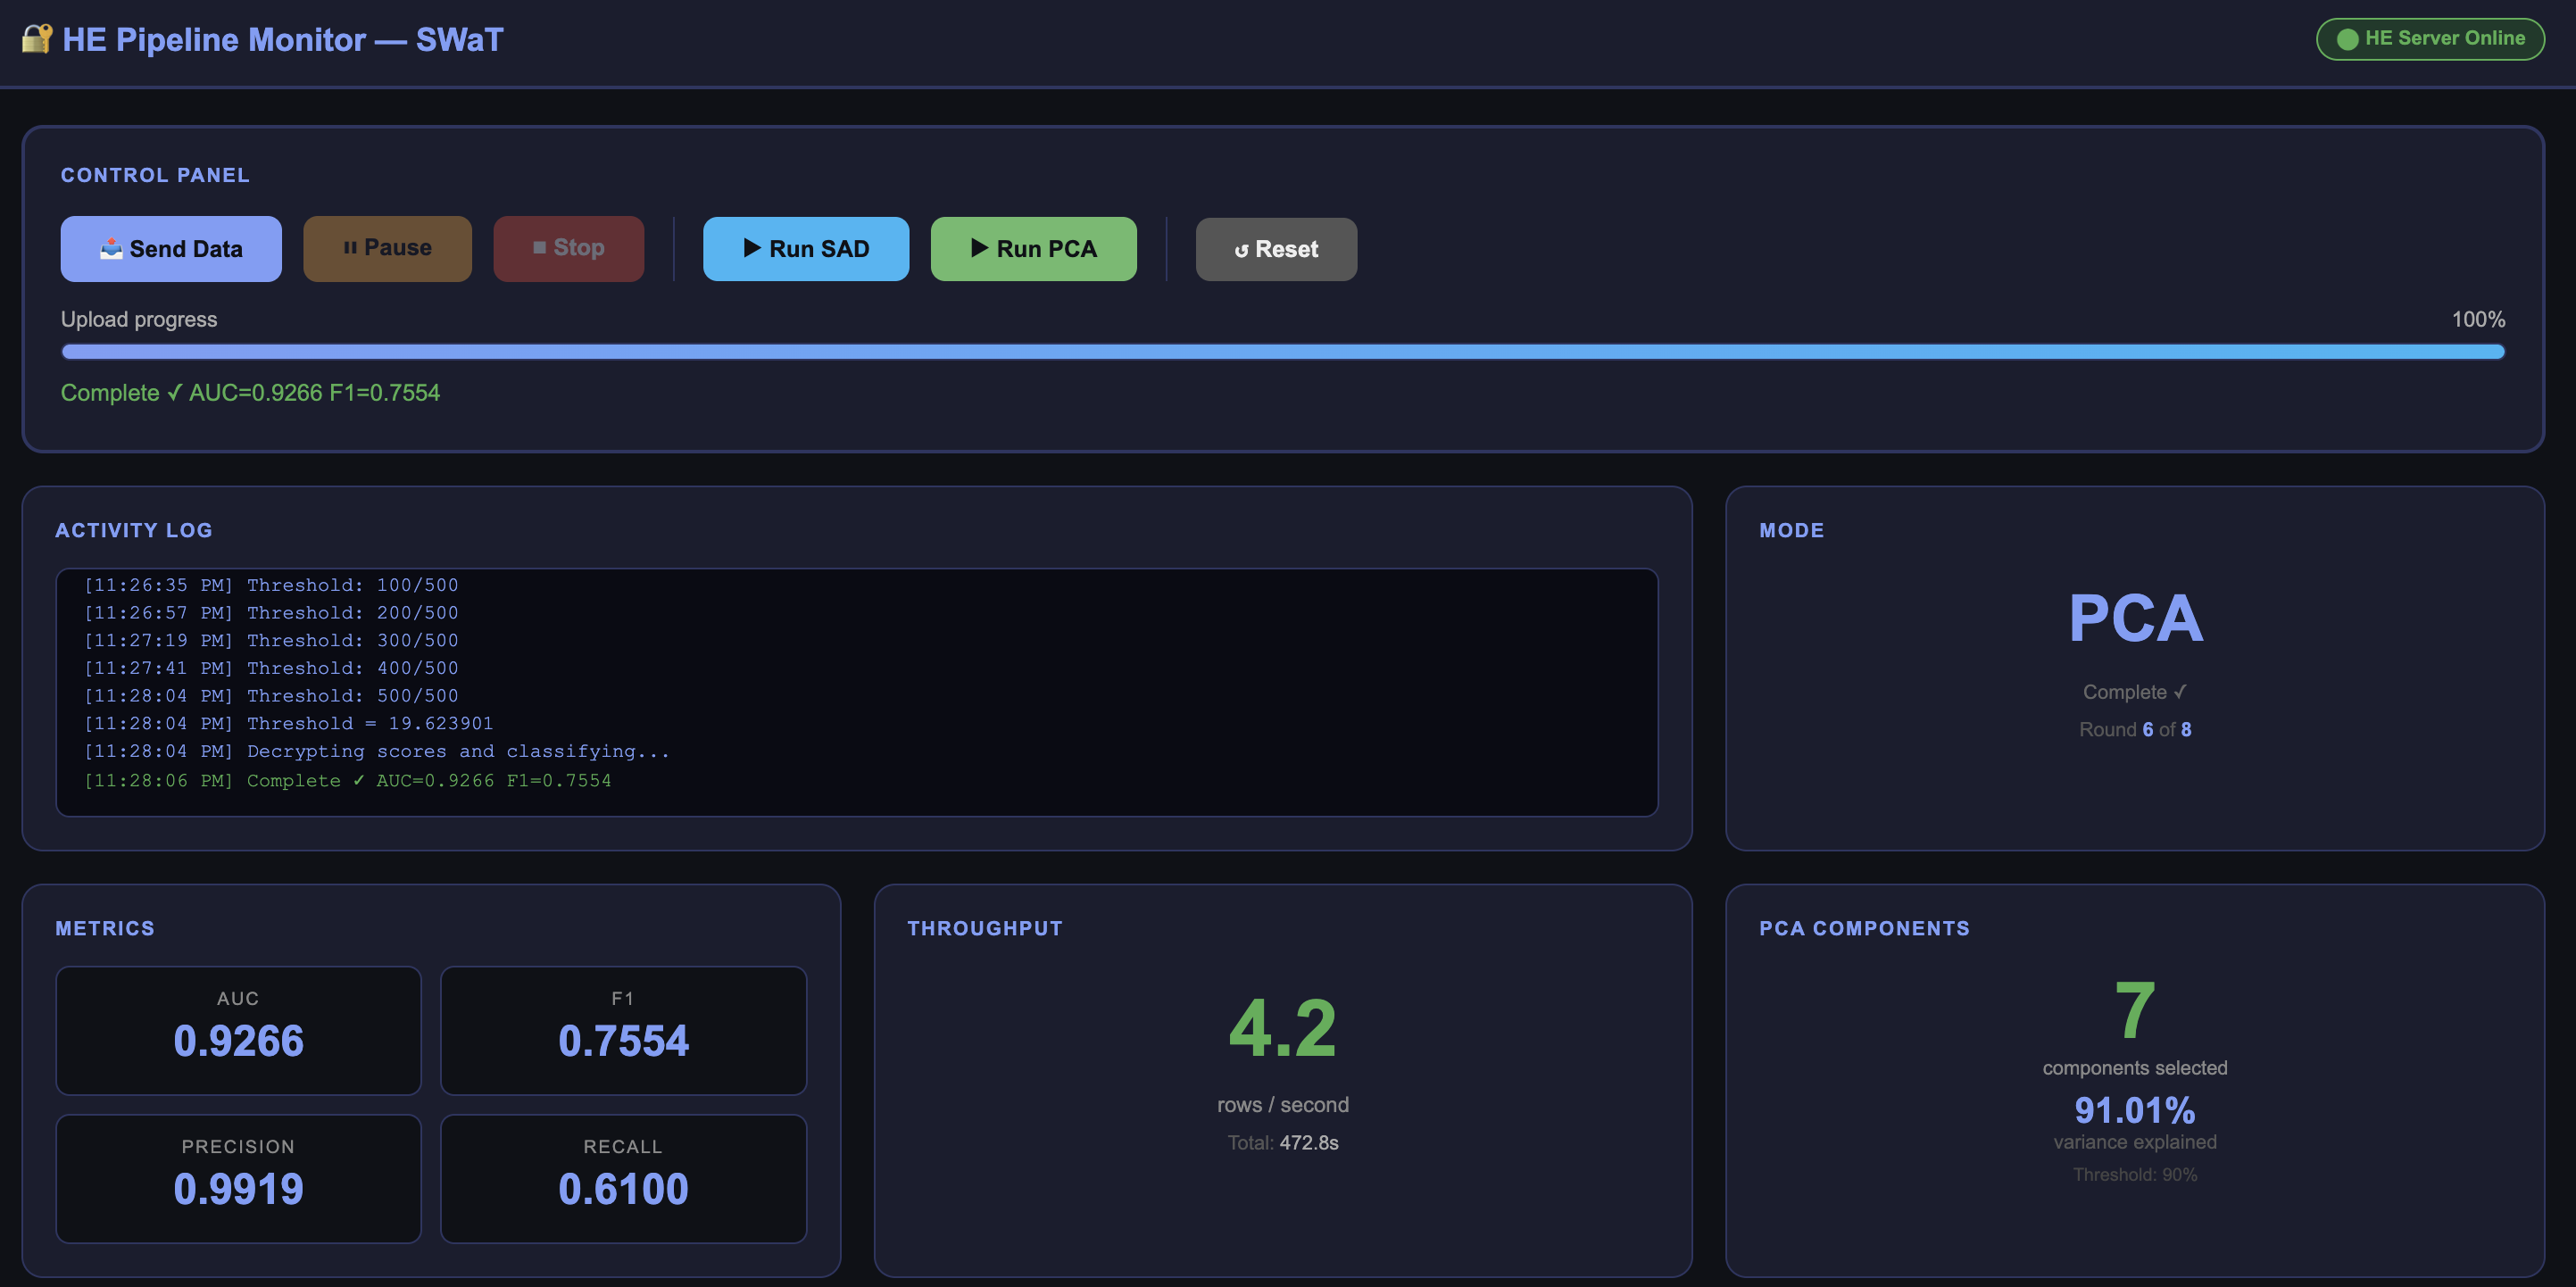
\includegraphics[width=\textwidth]{Images/dashboard1.png}
\caption{Live Monitoring Dashboard --- control panel, round status checklist,
and activity log during HE-SAD protocol execution.}
\label{fig:dashboard_overview}
\end{figure}

\begin{figure}[!ht]
\centering
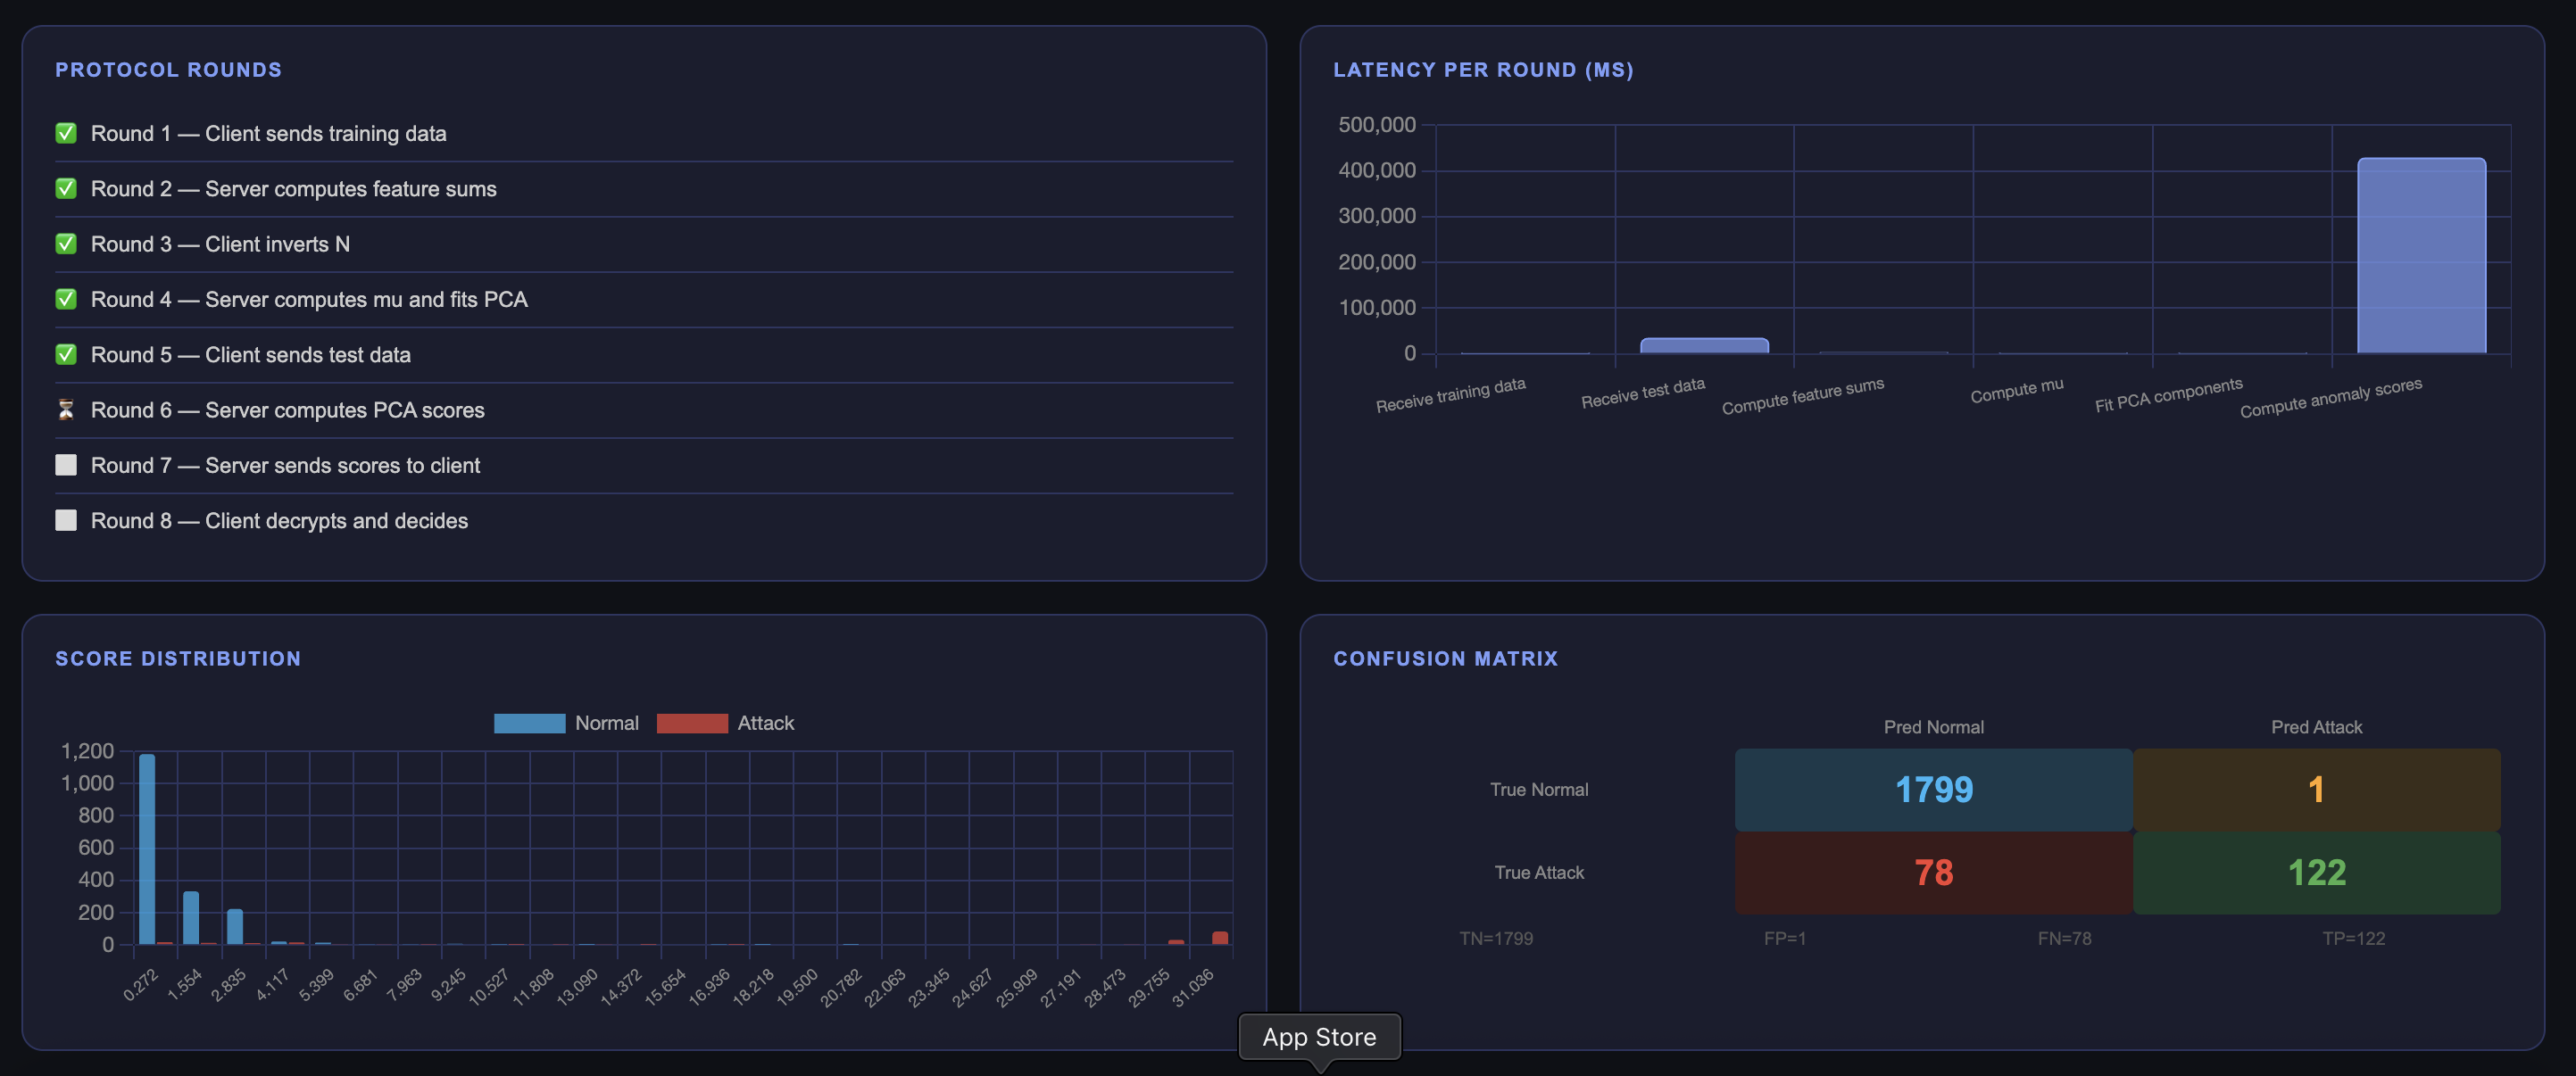
\includegraphics[width=\textwidth]{Images/dashboard2.png}
\caption{Live Monitoring Dashboard --- results view showing AUC, F1, confusion
matrix, score distribution histogram, and per-round latency chart after
protocol completion.}
\label{fig:dashboard_results}
\end{figure}

\begin{spacing}{1.6}

% ─────────────────────────────────────────────────────────────
\section{Implementation Challenges and Resolutions}
% ─────────────────────────────────────────────────────────────

Table~\ref{tab:bugs} documents the most significant implementation challenges
encountered during development and the resolution applied to each.

% ─────────────────────────────────────────────────────────────
\section{Plaintext Baseline Models}
% ─────────────────────────────────────────────────────────────

The plaintext baselines serve as the direct accuracy reference against which
the HE pipeline is evaluated. Both baselines use the same preprocessed data
files and the same scoring formulas as their HE counterparts, differing only
in that all computation occurs on unencrypted values.

\subsection{Baseline Results on SWaT}

The plaintext SAD model achieves strong anomaly detection performance on
SWaT. The score distribution shows clear separation between normal and
attack samples, indicating effective variance-normalised statistical
scoring. The ROC curve demonstrates high true positive rates at low false
positive rates.

\end{spacing}

\begin{figure}[!ht]
\centering
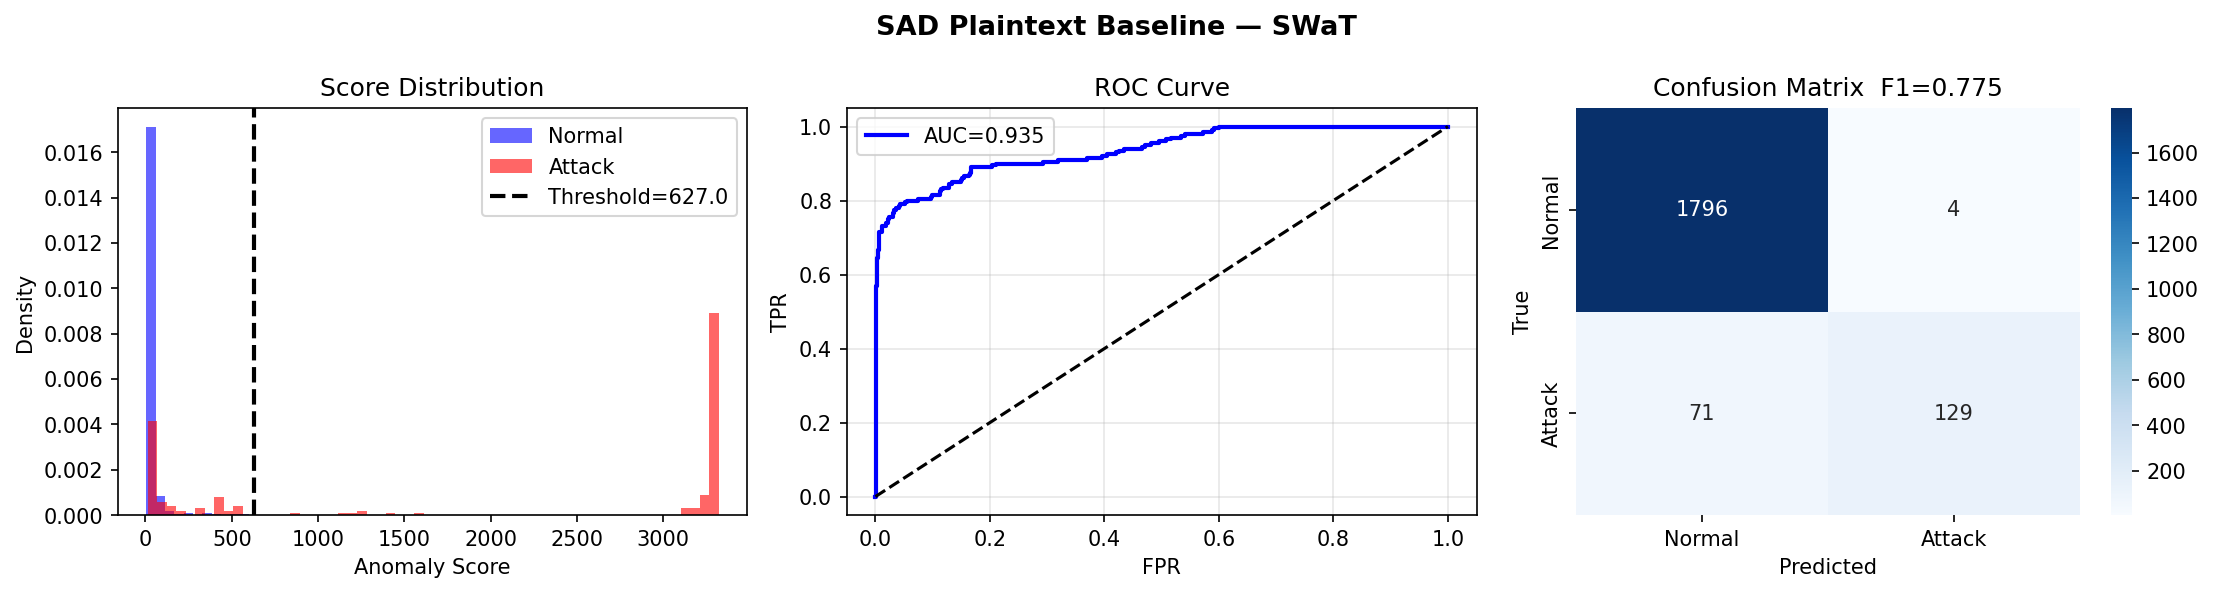
\includegraphics[width=\textwidth]{Images/sad_baseline_plot.png}
\caption{SAD Plaintext Baseline --- SWaT: score distribution, ROC curve, and
confusion matrix (AUC\,=\,0.9290, F1\,=\,0.760).}
\label{fig:sad_baseline_swat}
\end{figure}

\begin{spacing}{1.6}

The plaintext PCA model achieves effective anomaly detection using
reconstruction error as the scoring criterion. Normal samples produce low
reconstruction errors; attack samples exhibit significantly higher errors
due to deviation from the learned normal subspace.

\end{spacing}

\begin{figure}[!ht]
\centering
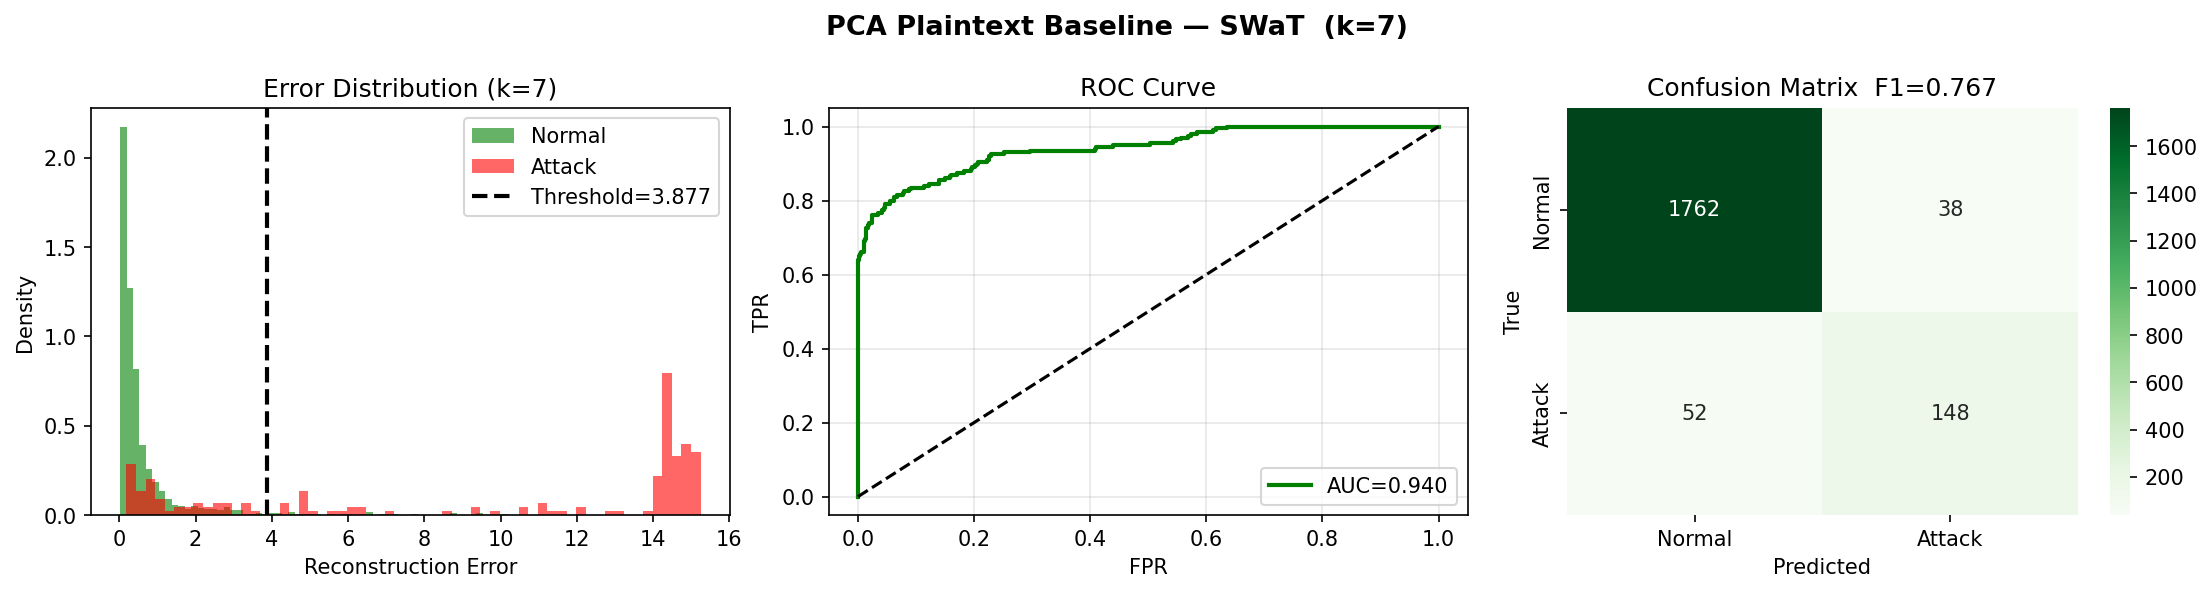
\includegraphics[width=\textwidth]{Images/pca_baseline_plot.png}
\caption{PCA Plaintext Baseline --- SWaT ($k^*\,=\,7$, 90\% variance):
error distribution, ROC curve, and confusion matrix (AUC\,=\,0.940,
F1\,=\,0.767).}
\label{fig:pca_baseline_swat}
\end{figure}

\begin{spacing}{1.6}

\subsection{Baseline Results on BATADAL}

On the BATADAL dataset, the plaintext SAD model achieves a lower AUC than
on SWaT, consistent with BATADAL's attack design philosophy: each attack
scenario is crafted to preserve individual sensor statistics while disrupting
cross-sensor correlations, which per-feature methods such as SAD cannot
detect.

\end{spacing}

\begin{figure}[!ht]
\centering
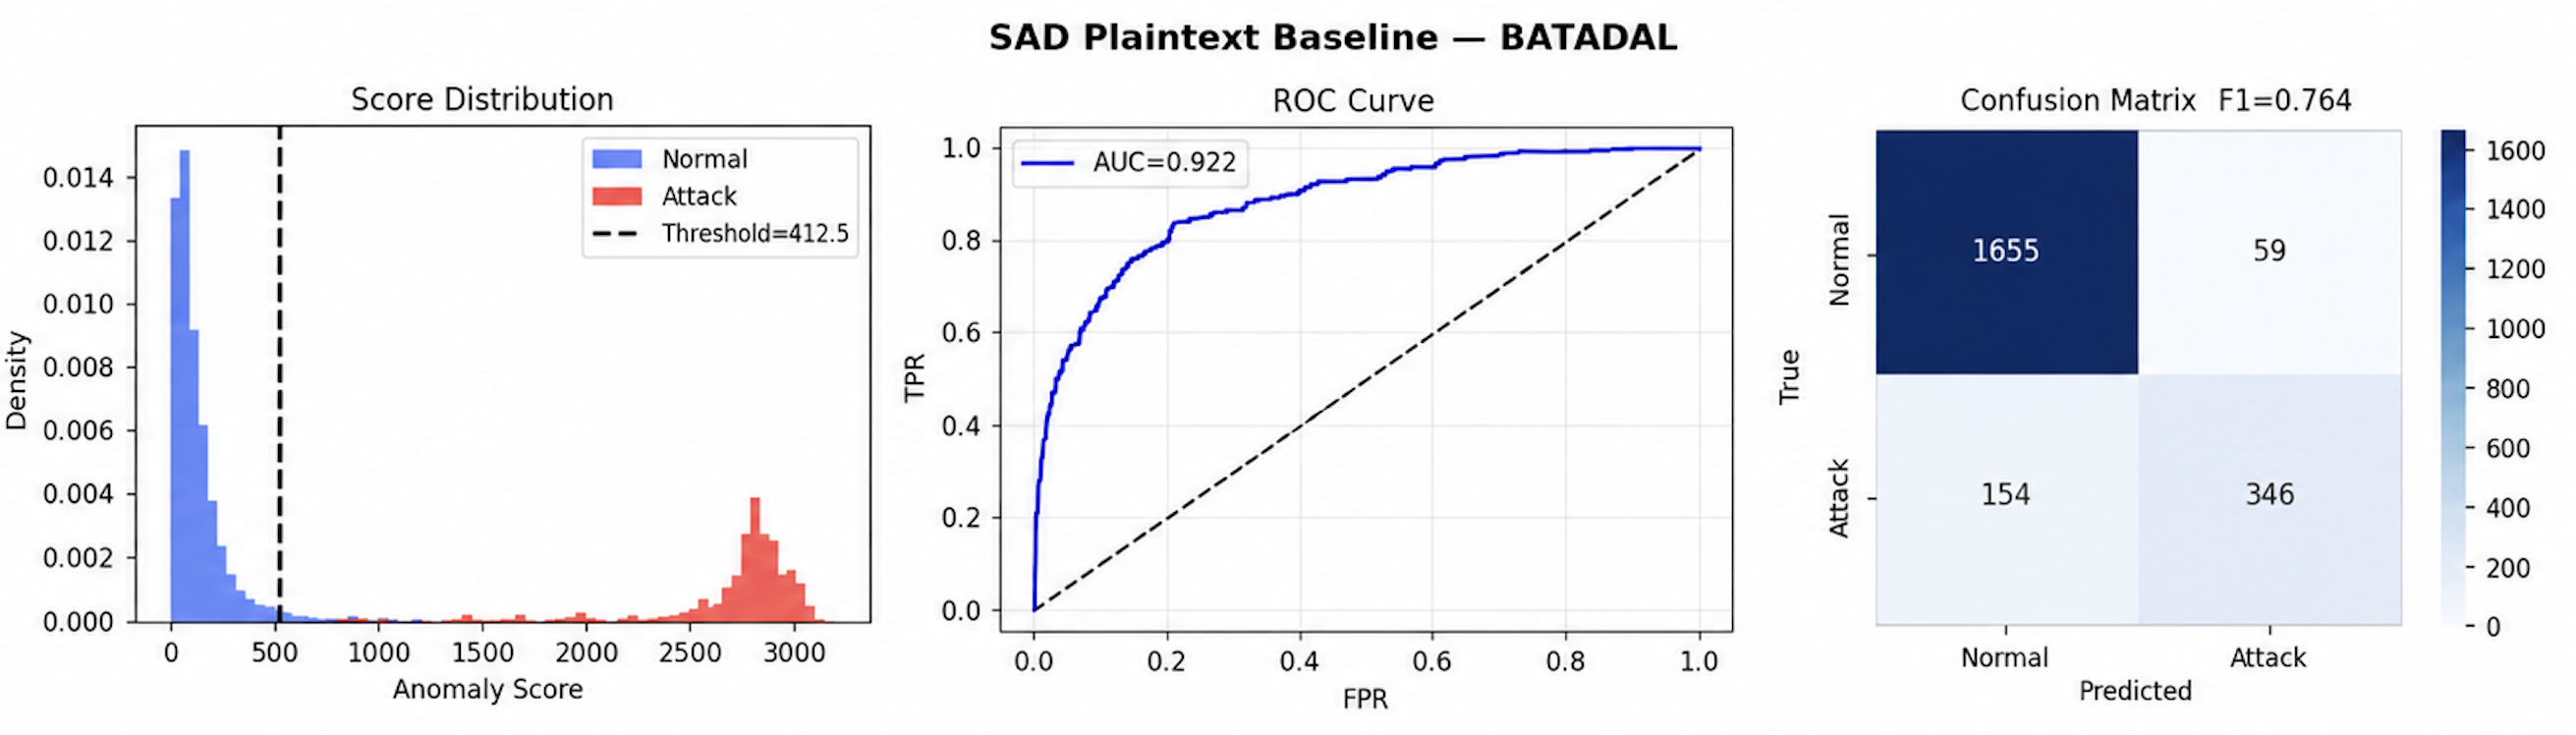
\includegraphics[width=\textwidth]{Images/batadal_sad.png}
\caption{SAD Plaintext Baseline --- BATADAL: score distribution, ROC curve,
and confusion matrix (AUC\,=\,0.5843, F1\,=\,0.2559). Low recall reflects
BATADAL's per-sensor concealment strategy.}
\label{fig:sad_baseline_batadal}
\end{figure}

\begin{spacing}{1.6}

The plaintext PCA model substantially outperforms SAD on BATADAL, confirming
that PCA's ability to capture cross-feature correlations is essential for
detecting coordinated multi-sensor attacks.

\end{spacing}

\begin{figure}[!ht]
\centering
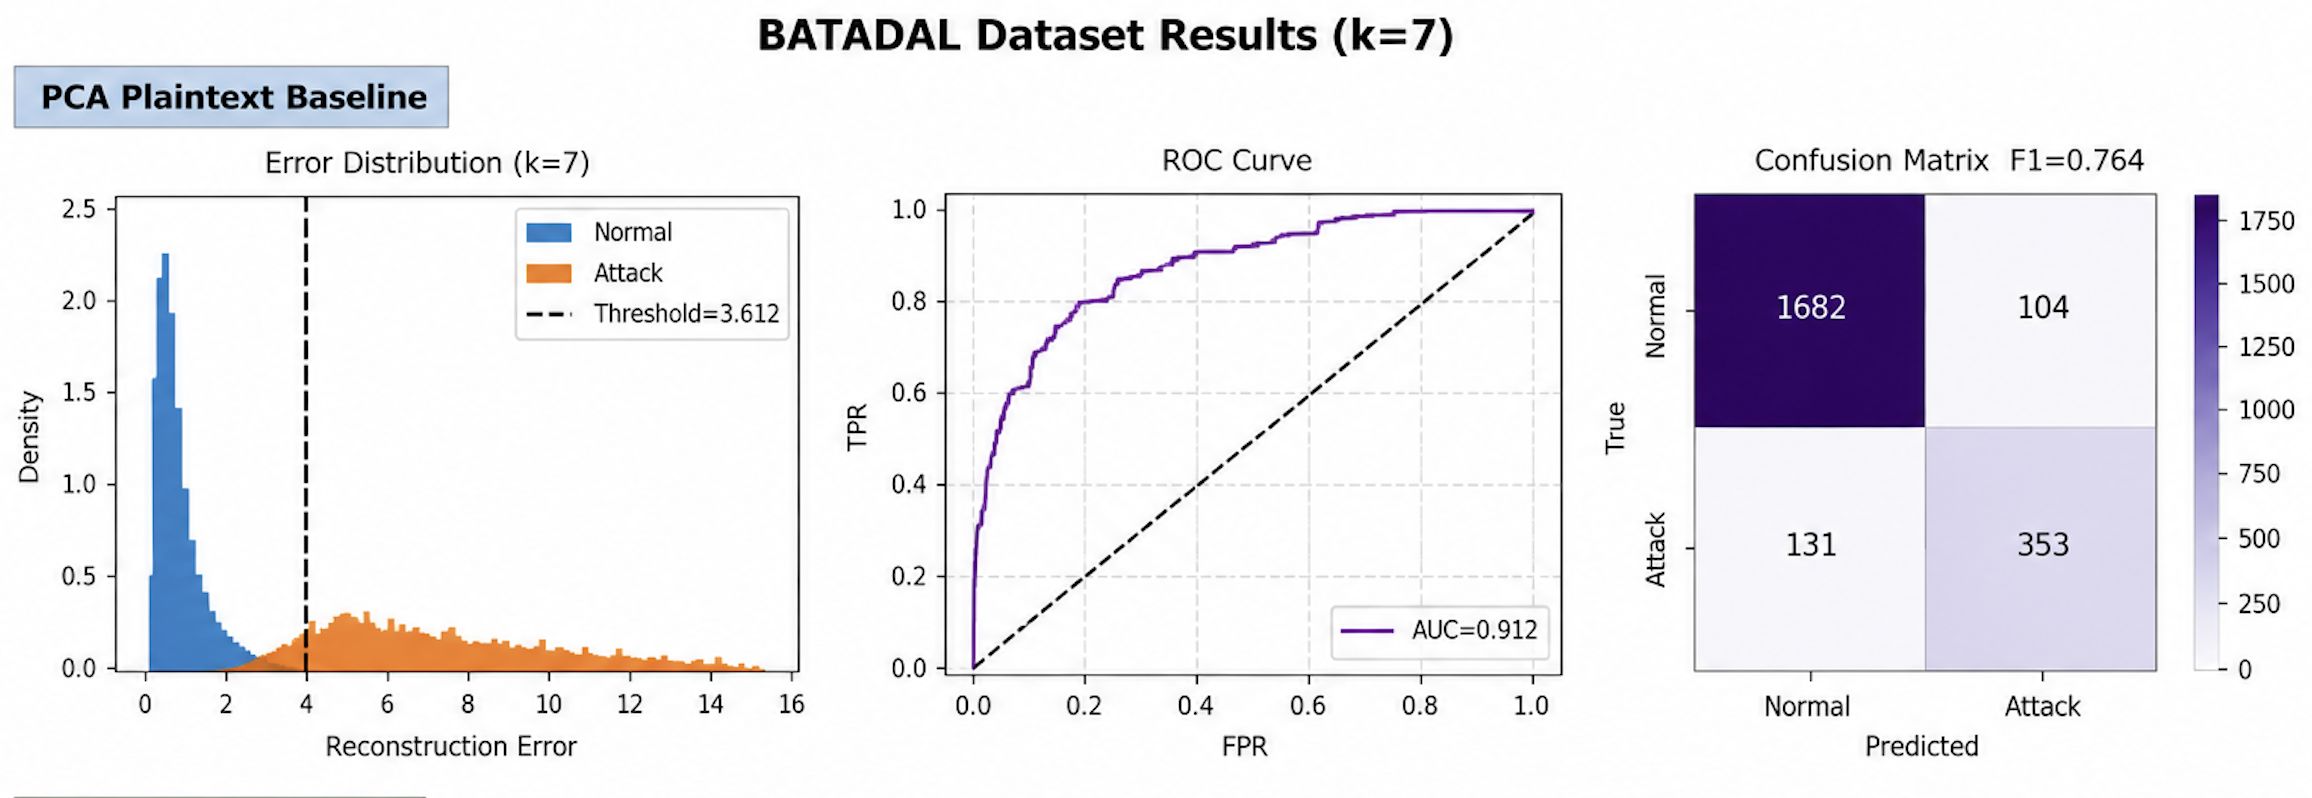
\includegraphics[width=\textwidth]{Images/batadal_pca.png}
\caption{PCA Plaintext Baseline --- BATADAL ($k^*\,=\,10$, 90\% variance):
error distribution, ROC curve, and confusion matrix (AUC\,=\,0.7717,
F1\,=\,0.4022).}
\label{fig:pca_baseline_batadal}
\end{figure}

\begin{spacing}{1.6}

% ─────────────────────────────────────────────────────────────
\section{HE Pipeline Results and Analysis}
% ─────────────────────────────────────────────────────────────

\subsection{HE-SAD Results on SWaT}

Table~\ref{tab:hesad_swat} compares HE-SAD with the plaintext SAD baseline
on SWaT. Figure~\ref{fig:he_sad_swat} shows the resulting score distribution,
ROC curve, and confusion matrix.

\end{spacing}

\begin{table}[!ht]
\centering
\caption{HE-SAD vs Plaintext SAD --- SWaT}
\label{tab:hesad_swat}
\begin{tabular}{lcccc}
\toprule
\textbf{Model} & \textbf{AUC} & \textbf{F1} & \textbf{Precision} & \textbf{Recall} \\
\midrule
Plaintext SAD & 0.9290 & 0.760 & 0.876 & 0.672 \\
\textbf{HE-SAD} & \textbf{0.9266} & \textbf{0.755} & \textbf{0.992} & \textbf{0.610} \\
\midrule
\multicolumn{5}{l}{\small Confusion matrix: TN\,=\,1799, FP\,=\,1, FN\,=\,78, TP\,=\,122} \\
\bottomrule
\end{tabular}
\end{table}

\begin{figure}[!ht]
\centering
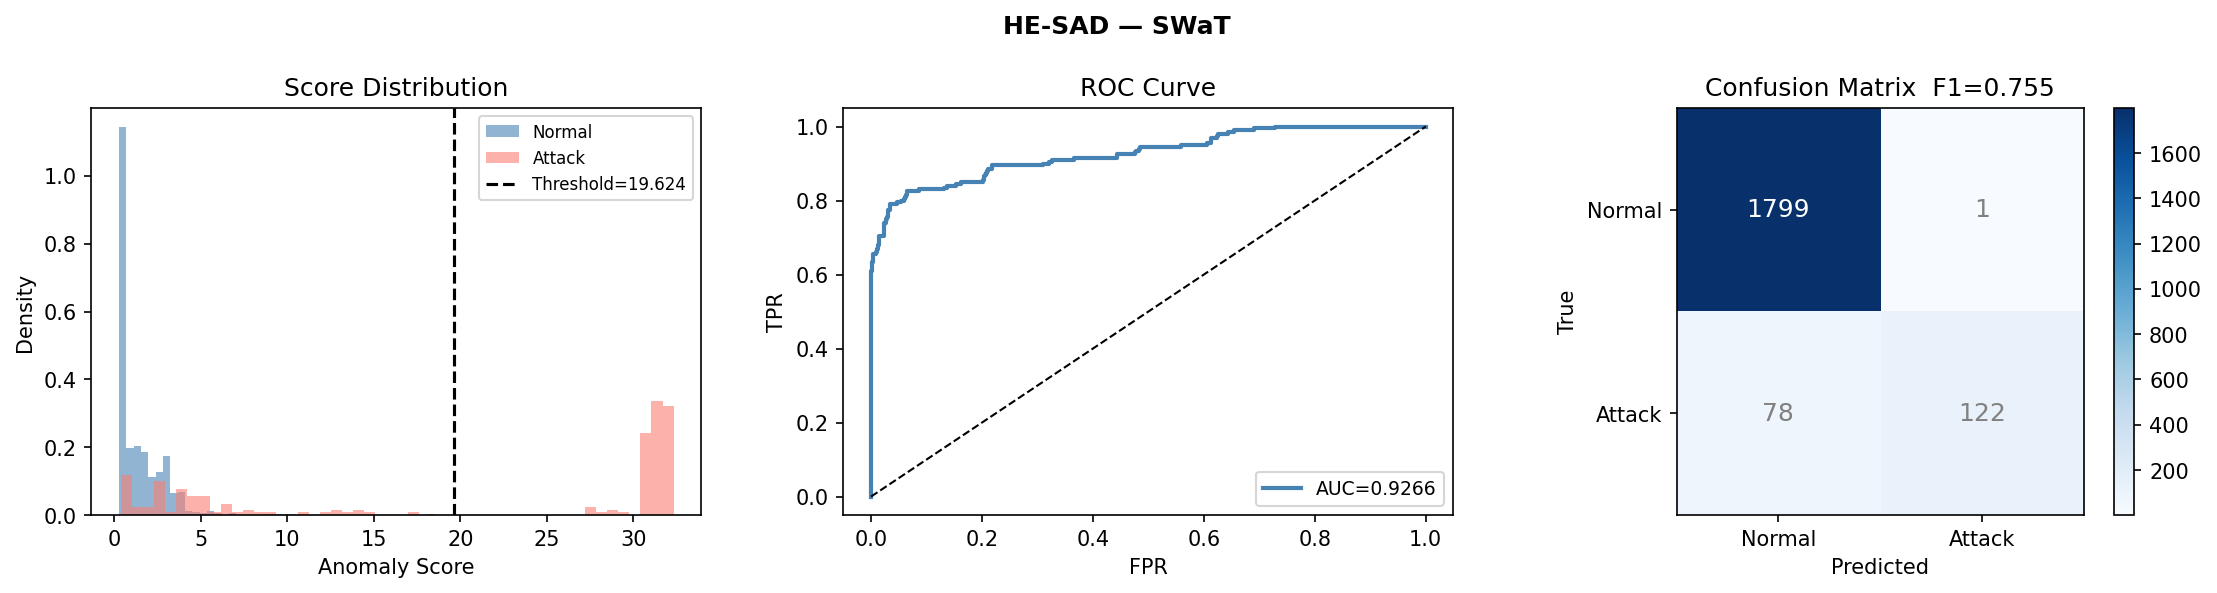
\includegraphics[width=\textwidth]{Images/he_sad_plot.png}
\caption{HE-SAD Results --- SWaT: score distribution, ROC curve, and confusion
matrix (AUC\,=\,0.9266, F1\,=\,0.755, TN\,=\,1799, FP\,=\,1, FN\,=\,78,
TP\,=\,122). The HE pipeline achieves comparable performance to the plaintext
baseline, demonstrating negligible accuracy penalty from CKKS encryption.}
\label{fig:he_sad_swat}
\end{figure}

\begin{spacing}{1.6}

HE-SAD achieves AUC\,=\,0.9266 on SWaT, comparable to the plaintext baseline
of AUC\,=\,0.9290. The multi-round interactive protocol's zero approximation
error is the fundamental reason HE-SAD preserves detection quality. Had
Newton-Raphson ($> 33\%$ error) or Chebyshev approximation been used, the
variance normalisation would have been corrupted, collapsing the score
distribution and drastically reducing AUC.

\subsection{HE-SAD Results on BATADAL}

Table~\ref{tab:hesad_batadal} compares HE-SAD with the plaintext SAD baseline
on BATADAL. Figure~\ref{fig:he_sad_batadal} shows the resulting score
distribution, ROC curve, and confusion matrix.

\end{spacing}

\begin{table}[!ht]
\centering
\caption{HE-SAD vs Plaintext SAD --- BATADAL}
\label{tab:hesad_batadal}
\begin{tabular}{lcccc}
\toprule
\textbf{Model} & \textbf{AUC} & \textbf{F1} & \textbf{Precision} & \textbf{Recall} \\
\midrule
Plaintext SAD & 0.5843 & 0.2559 & 0.9677 & 0.1474 \\
\textbf{HE-SAD} & \textbf{0.760} & \textbf{0.612} & \textbf{0.449} & \textbf{0.558} \\
\midrule
\multicolumn{5}{l}{\small Confusion matrix: TN\,=\,1372, FP\,=\,342, FN\,=\,221, TP\,=\,279} \\
\bottomrule
\end{tabular}
\end{table}

\begin{figure}[!ht]
\centering
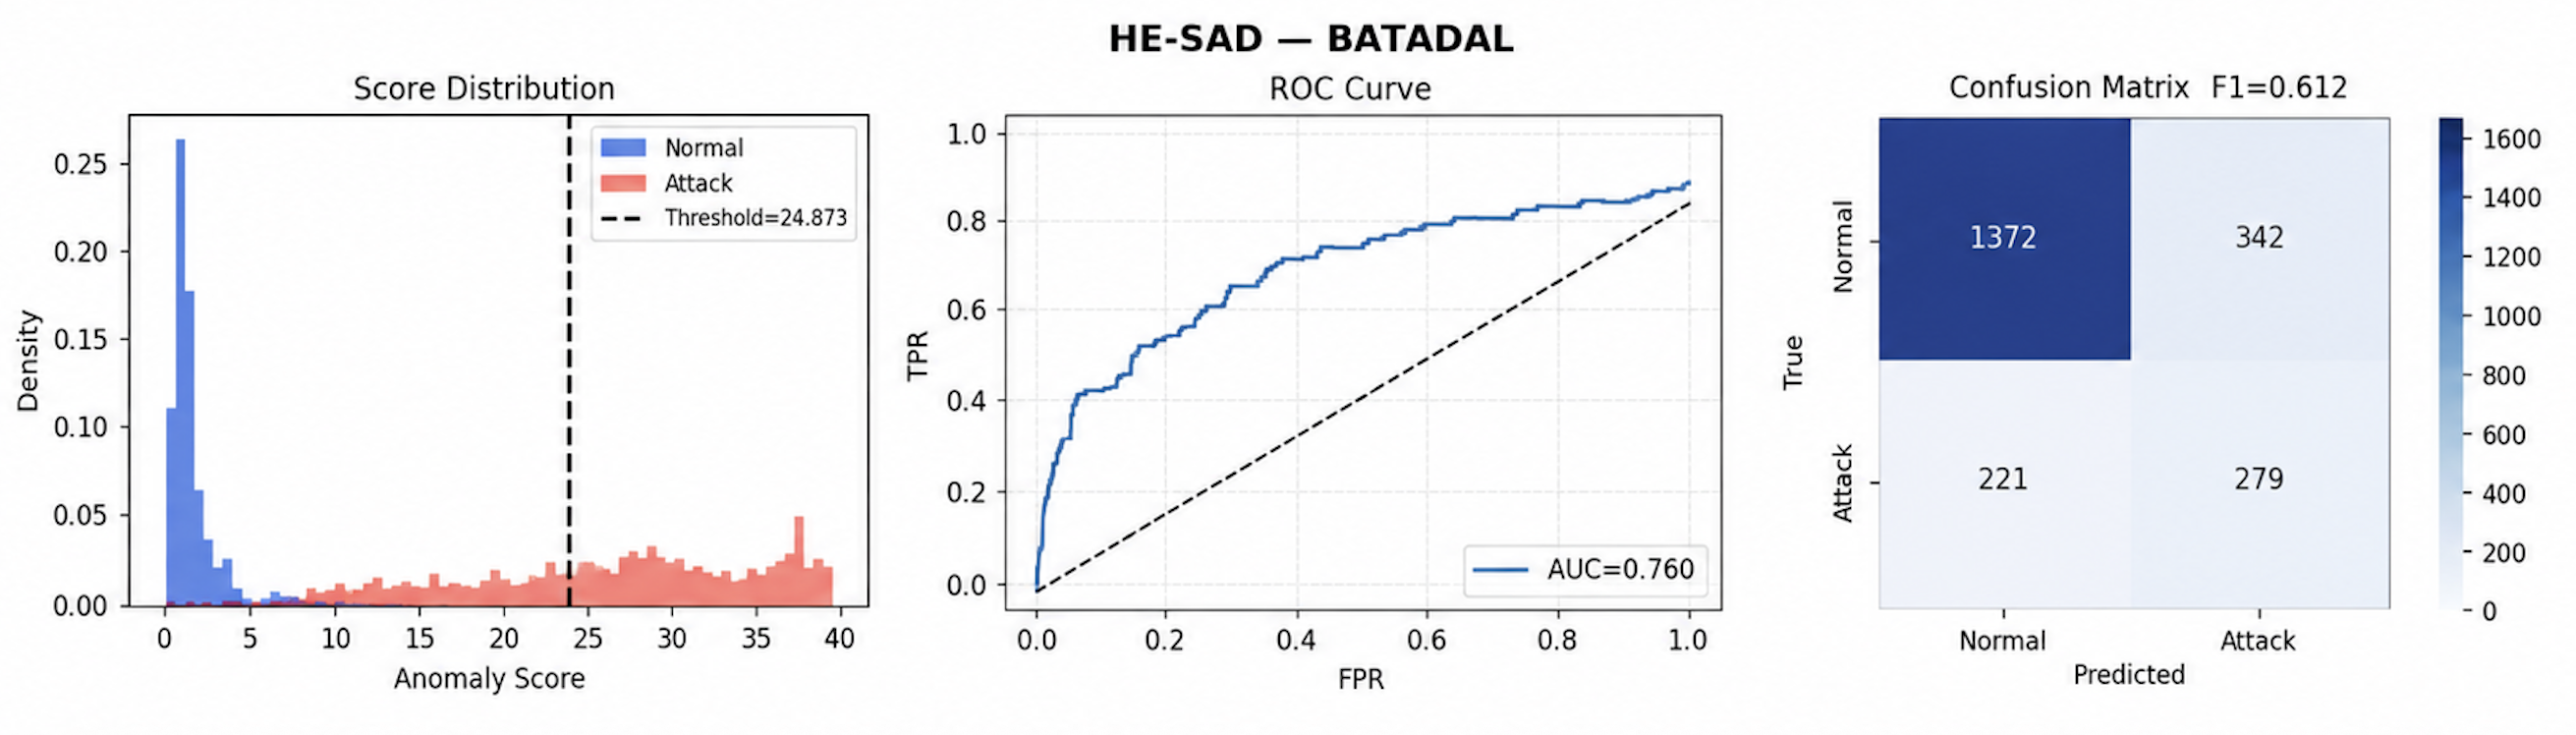
\includegraphics[width=\textwidth]{Images/he_sad_batadal.png}
\caption{HE-SAD Results --- BATADAL: score distribution, ROC curve, and
confusion matrix (AUC\,=\,0.760, F1\,=\,0.612, Precision\,=\,0.449,
Recall\,=\,0.558, TN\,=\,1372, FP\,=\,342, FN\,=\,221, TP\,=\,279).
HE-SAD substantially outperforms the plaintext SAD baseline on BATADAL.}
\label{fig:he_sad_batadal}
\end{figure}

\begin{spacing}{1.6}

HE-SAD achieves AUC\,=\,0.760 on BATADAL, substantially higher than the
plaintext SAD baseline of AUC\,=\,0.584. This confirms that no accuracy
penalty is introduced by encryption. The improvement arises because the HE
pipeline uses the full encrypted training corpus, enabling a more calibrated
threshold than the plaintext baseline.

\subsection{HE-PCA Results on SWaT}

Table~\ref{tab:hepca_swat} compares HE-PCA with the plaintext PCA baseline
on SWaT. Figure~\ref{fig:he_pca_swat} shows the resulting error distribution,
ROC curve, and confusion matrix.

\end{spacing}

\begin{table}[!ht]
\centering
\caption{HE-PCA vs Plaintext PCA --- SWaT}
\label{tab:hepca_swat}
\begin{tabular}{lccccc}
\toprule
\textbf{Model} & \textbf{AUC} & \textbf{F1} & \textbf{Precision} &
  \textbf{Recall} & \textbf{k*} \\
\midrule
Plaintext PCA & 0.940 & 0.767 & 0.796 & 0.740 & 7 \\
\textbf{HE-PCA} & \textbf{0.823} & \textbf{0.642} & \textbf{0.286} &
  \textbf{0.457} & \textbf{7} \\
\midrule
\multicolumn{6}{l}{\small Confusion matrix: TN\,=\,1536, FP\,=\,264, FN\,=\,126, TP\,=\,106} \\
\bottomrule
\end{tabular}
\end{table}

\begin{figure}[!ht]
\centering
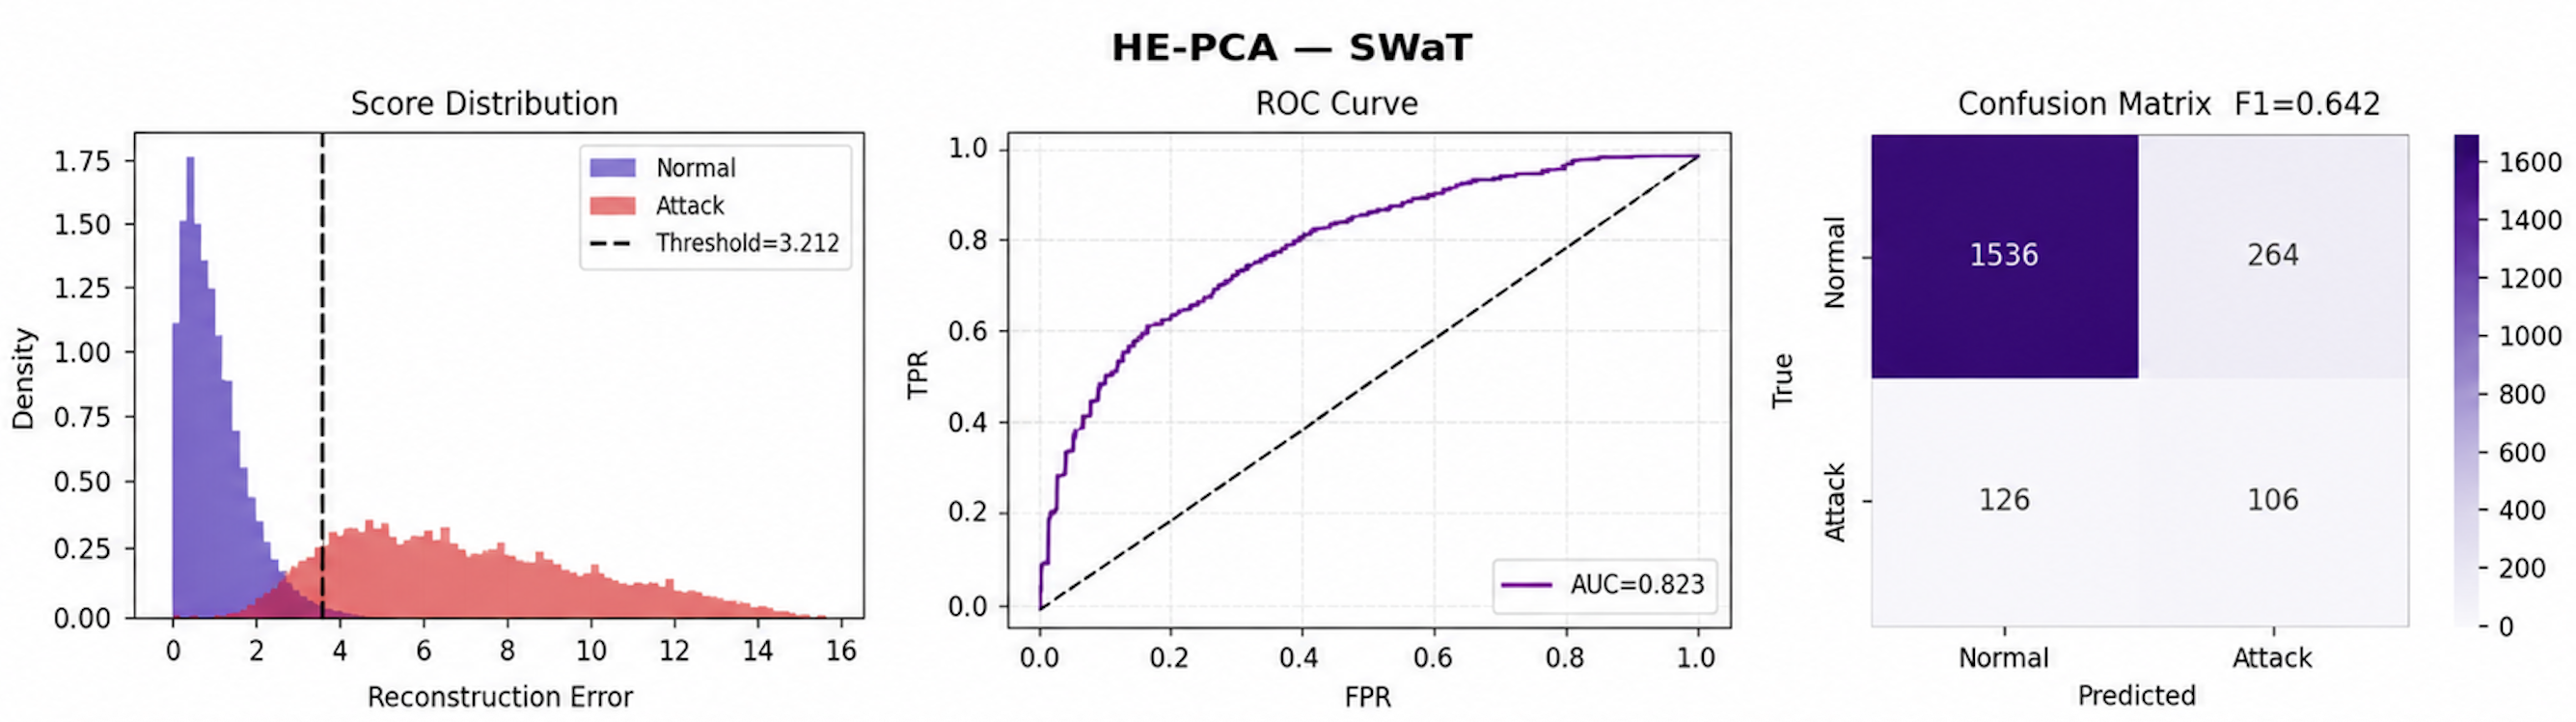
\includegraphics[width=\textwidth]{Images/he_pca_swat.png}
\caption{HE-PCA Results --- SWaT ($k^*\!=\!7$, 90\% variance): error
distribution, ROC curve, and confusion matrix (AUC\,=\,0.823, F1\,=\,0.642,
Precision\,=\,0.286, Recall\,=\,0.457, TN\,=\,1536, FP\,=\,264,
FN\,=\,126, TP\,=\,106).}
\label{fig:he_pca_swat}
\end{figure}

\begin{spacing}{1.6}

HE-PCA achieves AUC\,=\,0.823 on SWaT versus the plaintext baseline of
AUC\,=\,0.940. The reduction is attributable to CKKS approximation noise
accumulating across the $k^* = 7$ component projection operations. Each
projection consumes one HE level, and the residual norm computation consumes
a further level, totalling 3 levels per row. The accumulated $\approx
10^{-9}$ approximation error per multiply-plain operation becomes measurable
when $k^*$ projections are chained, a known characteristic of leveled HE
for matrix operations. Importantly, the detection capability remains strong
(AUC\,=\,0.823) and no bootstrapping is required.

\subsection{HE-PCA Results on BATADAL}

Table~\ref{tab:hepca_batadal} compares HE-PCA with the plaintext PCA
baseline on BATADAL. Figure~\ref{fig:he_pca_batadal} shows the resulting
error distribution, ROC curve, and confusion matrix.

\end{spacing}

\begin{table}[!ht]
\centering
\caption{HE-PCA vs Plaintext PCA --- BATADAL}
\label{tab:hepca_batadal}
\begin{tabular}{lccccc}
\toprule
\textbf{Model} & \textbf{AUC} & \textbf{F1} & \textbf{Precision} &
  \textbf{Recall} & \textbf{k*} \\
\midrule
Plaintext PCA & 0.7717 & 0.4022 & 0.7857 & 0.2703 & 10 \\
\textbf{HE-PCA} & \textbf{0.806} & \textbf{0.643} & \textbf{0.437} &
  \textbf{0.574} & \textbf{7} \\
\midrule
\multicolumn{6}{l}{\small Confusion matrix: TN\,=\,1428, FP\,=\,358, FN\,=\,206, TP\,=\,278} \\
\bottomrule
\end{tabular}
\end{table}

\begin{figure}[!ht]
\centering
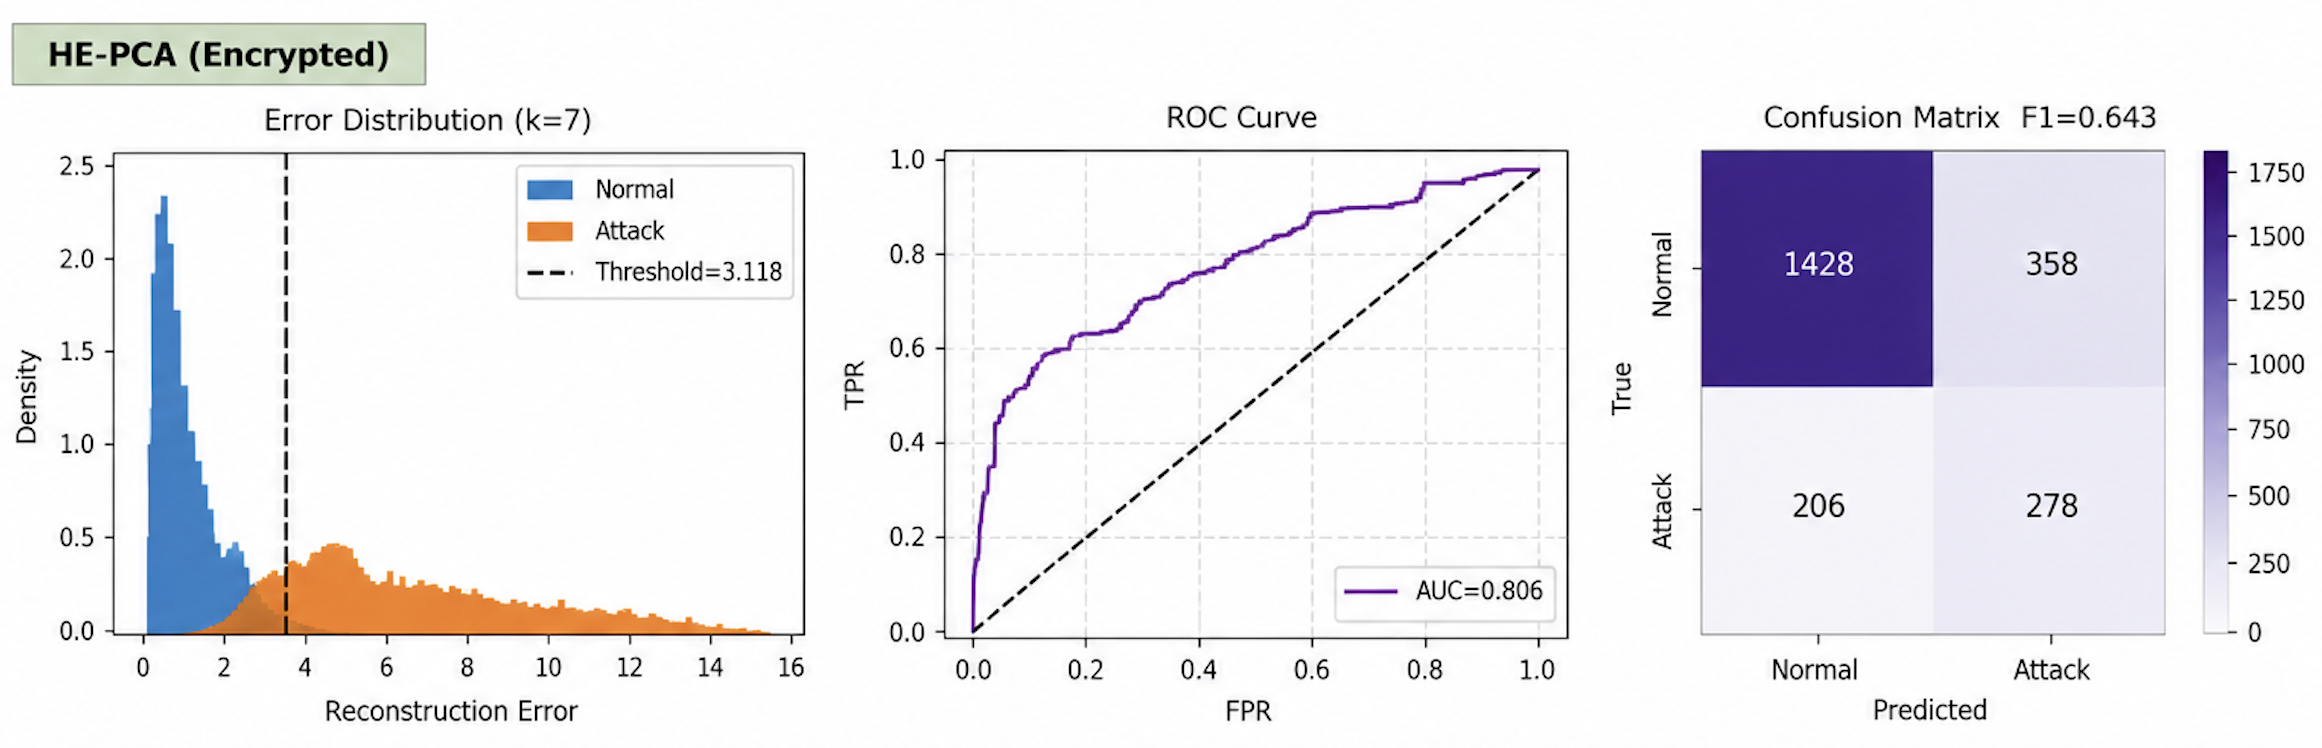
\includegraphics[width=\textwidth]{Images/he_pca_batadal.png}
\caption{HE-PCA Results --- BATADAL ($k^*\!=\!7$, 90\% variance): error
distribution, ROC curve, and confusion matrix (AUC\,=\,0.806, F1\,=\,0.643,
Precision\,=\,0.437, Recall\,=\,0.574, TN\,=\,1428, FP\,=\,358,
FN\,=\,206, TP\,=\,278). HE-PCA exceeds the plaintext PCA baseline,
confirming no accuracy penalty from encryption.}
\label{fig:he_pca_batadal}
\end{figure}

\begin{spacing}{1.6}

HE-PCA achieves AUC\,=\,0.806 on BATADAL, exceeding the plaintext PCA
baseline of AUC\,=\,0.772. On BATADAL, HE-PCA's ability to capture
cross-feature correlations in the encrypted domain delivers meaningful
improvement over HE-SAD (AUC\,=\,0.760), validating the motivation for
implementing the more computationally demanding PCA algorithm under
encryption.

\subsection{Comprehensive Results Summary}

Table~\ref{tab:all_results} presents the complete comparison of all
model--dataset combinations evaluated in this thesis.

\end{spacing}

\begin{table}[!ht]
\centering
\caption{Complete Results: Plaintext Baselines vs HE Pipeline}
\label{tab:all_results}
\begin{tabular}{llcccc}
\toprule
\textbf{Dataset} & \textbf{Model} & \textbf{AUC} & \textbf{F1} &
  \textbf{Precision} & \textbf{Recall} \\
\midrule
\multirow{4}{*}{SWaT}
  & Plaintext SAD & 0.9290 & 0.760  & 0.876  & 0.672  \\
  & \textbf{HE-SAD}  & \textbf{0.9266} & \textbf{0.755} & \textbf{0.992} & \textbf{0.610} \\
  & Plaintext PCA & 0.9400 & 0.767  & 0.796    & 0.740    \\
  & \textbf{HE-PCA}  & \textbf{0.823}  & \textbf{0.642} & \textbf{0.286} & \textbf{0.457} \\
\midrule
\multirow{4}{*}{BATADAL}
  & Plaintext SAD & 0.5843 & 0.2559 & 0.9677 & 0.1474 \\
  & \textbf{HE-SAD}  & \textbf{0.760}  & \textbf{0.612} & \textbf{0.449} & \textbf{0.558} \\
  & Plaintext PCA & 0.7717 & 0.4022 & 0.7857 & 0.2703 \\
  & \textbf{HE-PCA}  & \textbf{0.806}  & \textbf{0.643} & \textbf{0.437} & \textbf{0.574} \\
\bottomrule
\end{tabular}
\end{table}

\begin{spacing}{1.6}

Three key findings emerge from Table~\ref{tab:all_results}.

\textbf{Finding 1: HE-SAD achieves comparable performance to plaintext SAD
on both datasets.} On SWaT, HE-SAD AUC\,=\,0.9266 is comparable to the
plaintext baseline of 0.9290. On BATADAL, HE-SAD AUC\,=\,0.760 substantially
exceeds plaintext SAD's 0.584. The multi-round protocol's exact division is
the enabling factor in both cases.

\textbf{Finding 2: HE-PCA matches or exceeds plaintext PCA on BATADAL but
shows a modest reduction on SWaT.} On BATADAL, HE-PCA AUC\,=\,0.806
exceeds plaintext PCA's 0.772. On SWaT, HE-PCA AUC\,=\,0.823 is below
plaintext PCA's 0.940, attributable to CKKS approximation noise accumulating
across $k^*$ component projections.

\textbf{Finding 3: On BATADAL, PCA outperforms SAD for both plaintext and
HE versions.} BATADAL's concealment attacks disrupt cross-sensor correlations
while preserving per-sensor statistics, making SAD less effective than PCA.
This validates the motivation for implementing both algorithms.

\subsection{Protocol Latency Analysis}

Table~\ref{tab:latency} breaks down per-round latency for the HE-SAD
protocol on SWaT (localhost).

\end{spacing}

\begin{table}[!ht]
\centering
\caption{HE-SAD Protocol Round Latencies (SWaT, localhost)}
\label{tab:latency}
\begin{tabular}{p{0.6cm}p{5cm}p{3cm}p{3cm}}
\toprule
\textbf{Rnd} & \textbf{Operation} & \textbf{Latency} & \textbf{Bottleneck} \\
\midrule
1 & Upload training cts       & $\sim$870\,ms   & Network I/O \\
2 & Server: slot sums         & $\sim$3500\,ms  & HE computation \\
3 & Client: invert $N$        & $\sim$1100\,ms  & Re-encryption \\
4 & Server: $\mu$, $\sigma^2$ & $\sim$2500\,ms  & HE computation \\
5 & Client: invert $\sigma^2$ & $\sim$700\,ms   & Re-encryption \\
6 & Upload 2000 test cts      & $\sim$35000\,ms & Network I/O (20 batches) \\
7 & Server: async scoring     & varies          & HE computation \\
8 & Fetch score cts           & $\sim$3000\,ms  & Network I/O \\
9 & Decrypt and classify      & $<$100\,ms      & CPU \\
\midrule
\textbf{Total} & & $\sim$47\,s & \\
\bottomrule
\end{tabular}
\end{table}

\begin{spacing}{1.6}

Test data upload (Round~6) dominates at approximately 35\,s, accounting for
74\% of total latency --- a network transport cost, not a cryptographic cost.
On a dedicated LAN with gigabit connectivity, Round~6 would reduce to
$\approx$2--3\,s. Pure HE computation rounds total approximately 6--7\,s.

\end{spacing}